%---------------------------------------------------------------------
%  Writeup of the improved search of Run II data for single top quark
%  production at DZero.
%  Started: Oct 2006
%  Authors: The Single Top Working Group
%---------------------------------------------------------------------
%

\appendix
\section*{Appendix 1 --- Trigger Definitions and Simulation}
\label{appendix-triggers}

\subsection{Trigger Definitions}
Trigger requirements for the electron and muon analysis channels are
shown in Tables~\ref{electronchan-triggers} and
\ref{muonchan-triggers}. More details about these triggers can be found in
Refs.~\cite{top_trigger_web,d0_note_4512,d0_note_4978}.

\begin{table}[!h!tbp]
\begin{center}
\begin{ruledtabular}
\begin{tabular}{lc||ccc} 
\multicolumn{5}{c}{\hspace{0.1in}\underline{Electron Channel Triggers}}\vspace{0.1in}\\
Trigger Version & Trigger Name & Level 1 Condition & Level 2 Condition
& Level 3 Condition \\
\hline
 v8.0 -- v9.0  & EM15\_2JT15        & CEM(1,10)CJT(2,5) & EM(0.85,10)JET(2,10) & SHT(1,15)JET(2,15)          \\
 v9.0 -- v10.0 & EM15\_2JT15        & CEM(1,10)CJT(2,5) & EM(0.85,10)JET(2,10) & SH(1,15)JET(2,15)           \\
v10.0 -- v11.0 & EM15\_2JT15        & CEM(1,10)CJT(2,5) & EM(0.85,10)JET(2,10) & SH(1,15)JET(2,15)           \\
v11.0 -- v12.0 & EM15\_2JT15        & CEM(1,10)CJT(2,5) & EM(0.85,10)JET(2,10) & SH(1,15)JET(2,15)           \\
v12.0 -- v13.0 & E1\_SHT15\_2J20    & CEM(1,11)         & None                 & SHT(1,15)JET(2,20)          \\
v13.0 -- v13.3 & E1\_SHT15\_2J\_J25 & CEM(1,11)         & L2CALEM(15,x)        & SHT(1,15)JET(1,25)JET(2,20) \\
v13.3 -- v14.0 & E1\_SHT15\_2J\_J30 & CEM(1,11)         & L2CALEM(15,x)        & SHT(1,15)JET(1,30)JET(2,20) \\
v14.0 -- v15.0 & E1\_SHT15\_2J\_J25 & CEM(1,12)         & L2CALEM(15,x)        & SHT(1,15)JET(1,25)JET(2,20)
\end{tabular}
\end{ruledtabular}
\vspace{-0.1in}
\caption[eltriggers]{Definitions of triggers used in the
electron channel of the single top analysis.}
\label{electronchan-triggers}
\end{center}
\end{table}

\vspace{-0.25in}

\begin{table}[!h!tbp]
\begin{center}
\begin{ruledtabular}
\begin{tabular}{lc||ccc} 
\multicolumn{5}{c}{\hspace{0.1in}\underline{Muon Channel Triggers}}\vspace{0.1in}\\
Trigger Version & Trigger Name & Level 1 Condition & Level 2 Condition & Level 3 Condition \\
\hline
 v8.0 -- v9.0  & MU\_JT20\_L2M0   & mu1ptxatxx\_CJT(1,5) & MUON(1,med)          & JET(1,20)                 \\
 v9.0 -- v10.0 & MU\_JT20\_L2M0   & mu1ptxatxx\_CJT(1,5) & MUON(1,med)          & JET(1,20)                 \\
v10.0 -- v11.0 & MU\_JT20\_L2M0   & mu1ptxatxx\_CJT(1,5) & MUON(1,med)          & JET(1,20)                 \\
v11.0 -- v12.0 & MU\_JT20\_L2M0   & mu1ptxatxx\_CJT(1,5) & MUON(1,med)          & JET(1,20)                 \\
v12.0 -- v13.0 & MU\_JT25\_L2M0   & mu1ptxatxx\_CJT(1,3) & MUON(1,med)JET(1,10) & JET(1,25)                 \\
v13.0 -- v13.2 & MUJ2\_JT25       & mu1ptxatxx\_CJT(1,5) & MUON(1,med)JET(1,8)  & JET(1,25)                 \\
v13.2 -- v13.3 & MUJ2\_JT25\_LM3  & mu1ptxatlx\_CJT(1,5) & MUON(1,med)JET(1,8)  & JET(1,25)MUON(1,3.,loose) \\
v13.3 -- v14.0 & MUJ2\_JT30\_LM3  & mu1ptxatlx\_CJT(1,5) & MUON(1,med)JET(1,8)  & JET(1,30)MUON(1,3.,loose) \\
v14.0 -- v14.2 & MUJ1\_JT25\_LM3  & mu1ptxatlx\_CJT(1,5) & MUON(1,med)JET(1,8)  & JET(1,25)MUON(1,3.,loose) \\
v14.2 -- v14.3 & MUJ1\_JT25\_ILM3 & mu1ptxatlx\_CJT(1,5) & MUON(1,med)JET(1,8)  & JET(1,25)MUON(1,3.,loose) \\
                                  &                      &                      & ISO\_MUON(1oose)          \\
v14.3 -- v15.0 & MUJ1\_JT35\_LM3  & mu1ptxatlx\_CJT(1,5) & MUON(1,med)JET(1,8)  & JET(1,35)MUON(1,3.,loose) \\
\end{tabular}
\end{ruledtabular}
\vspace{-0.1in}
\caption[muonchantriggers]{Definitions of triggers used in the
muon channel of the single top analysis.}
\label{muonchan-triggers}
\end{center}
\end{table}

\vspace{-0.2in}
For the electron channel at Level 1, trigger term CEM(1,X) requires
that events must contain at least one electromagnetic trigger tower
with transverse energy $E_T > X$~GeV where $X = 10, 11,$ or 12, and
trigger term CJT(2,5) requires that events must contain at least two
calorimeter jet trigger towers with energy above 5~GeV. At Level 2,
EM(0.85,10) requires at least one Level 2 electromagnetic object with
$E_T > 10$~GeV and electromagnetic fraction greater than 0.85,
JET(2,10) requires at least two Level 2 jets with $E_T > 10$~GeV, and
L2CALEM(15,x) requires a standard Level 2 EM cluster with $E_T >
15$~GeV. At Level 3, SH(1,15) (SHT(1,15)) requires at least one
electron defined with a (tight) shower shape cut and $E_T > 15$~GeV,
JET(1,X) (JET(2,X)) requires at least one (two) Level 3 jet(s) with
$E_T > X$~GeV where $X = 15, 20, 25,$ or 30.

For the muon channel at Level 1, trigger term mu1ptxatxx (mu1ptxatlx)
requires that events must fire the single-muon trigger based on muon
scintillators with no (loose) wires, and CJT(1,X) requires at least
one calorimeter jet trigger tower with $E_T > X$~GeV where $X = 3$ or
5. At Level 2, MUON(1,med) requires one muon candidate with medium
quality, and JET(1,X) requires at least one Level 2 jet with $E_T >
X$~GeV where $X = 8$ or 10. At Level 3, JET(1,X) requires at least one
Level 3 jet with $E_T > X$~GeV where $X = 20, 25, 30,$ or 35,
MUON(1,3.,loose) requires one muon candidate with loose quality and
$p_T > 3$~GeV, and ISO\_MUON(1,3,loose) requires one isolated muon
candidate with loose quality and $p_T > 3$~GeV. The presence of
two Level 2 trigger terms in the v14.2 list indicates that events must
fire either of these terms.

\subsection{Trigger Simulation in Monte Carlo}
\label{trigger-simulation}

Objects in Monte Carlo events need to have the trigger inefficiencies
simulated. We do this by modifying the weight for each MC event using
trigger efficiency turn-on curves for each object measured on
data. This method does not determine if a Monte Carlo event passes or
fails the trigger, instead the probability of that event to fire the
trigger is calculated.  Details of the method and its implementation
can be found in Ref.~\cite{d0_note_4512,d0_note_4882,caf_trigger}. An
example electron turn-on curve versus $p_T$ is shown in
Fig.~\ref{trigger-turnons} together with an example muon turn-on curve
versus {\deta}.

\begin{figure}[!h!tbp]
\begin{center}
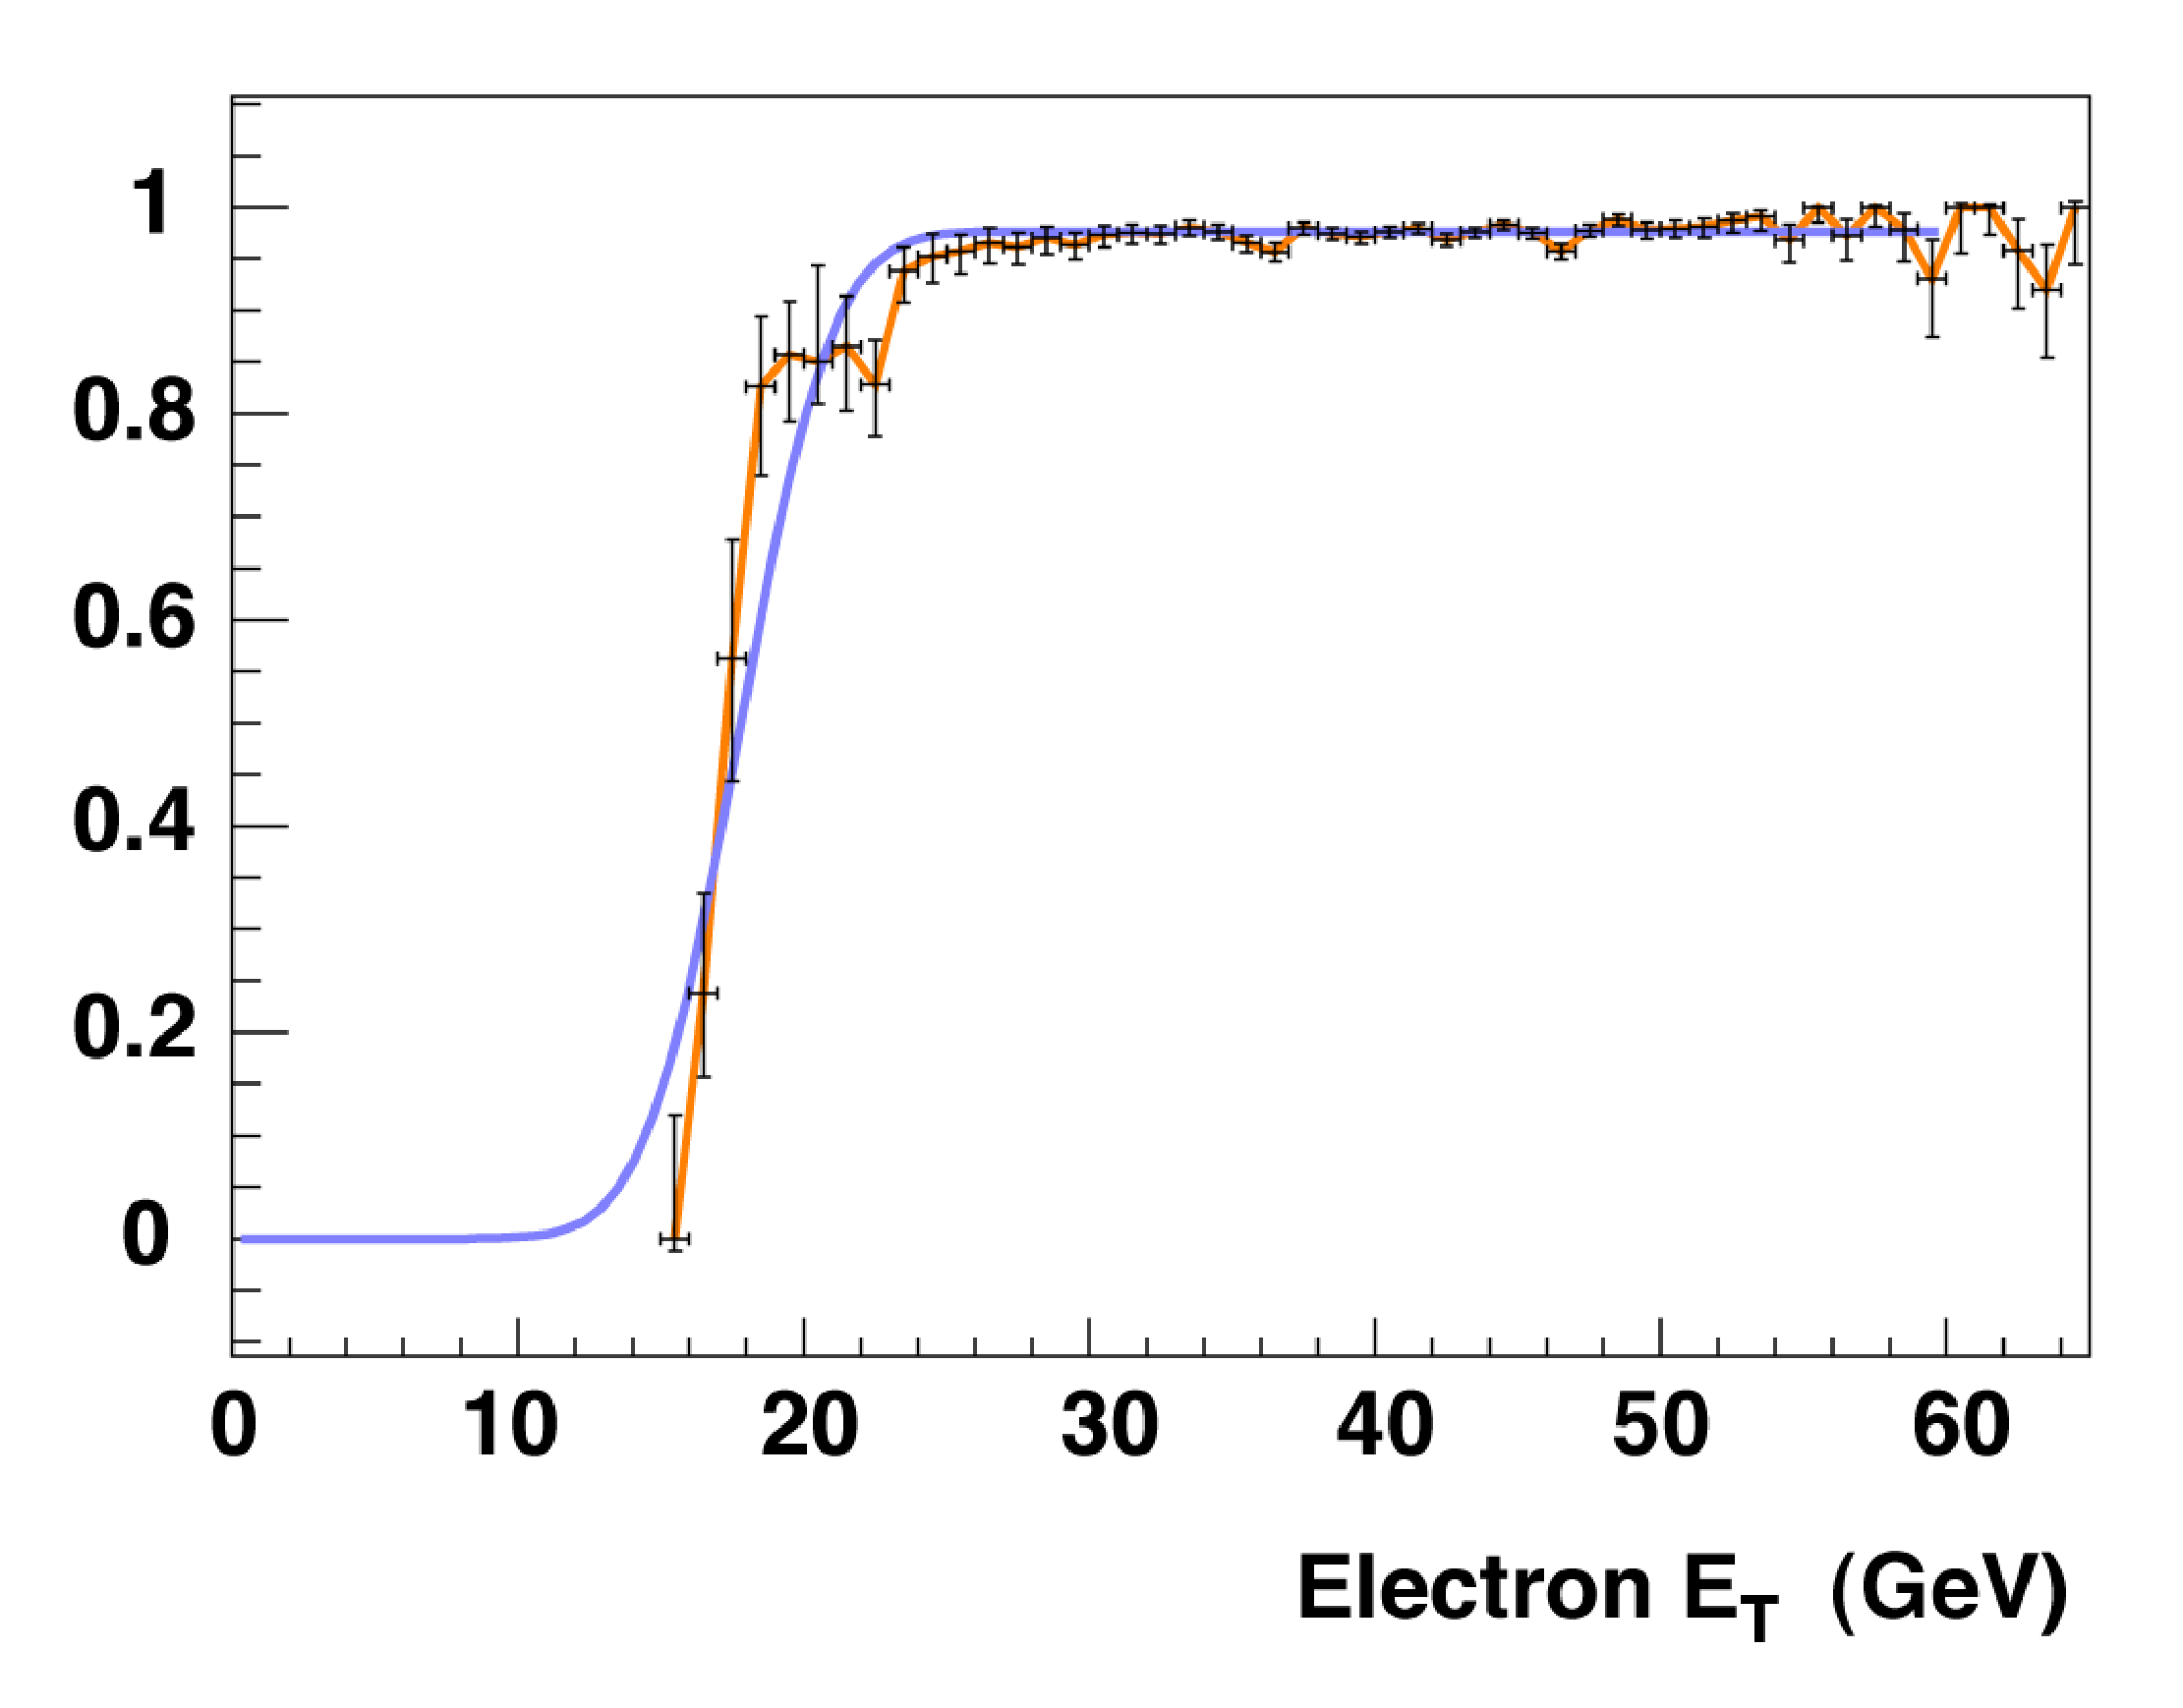
\includegraphics[width=0.35\textwidth]
{figures/electron_turn-on_curve_pt.eps}
\hspace{0.5in}
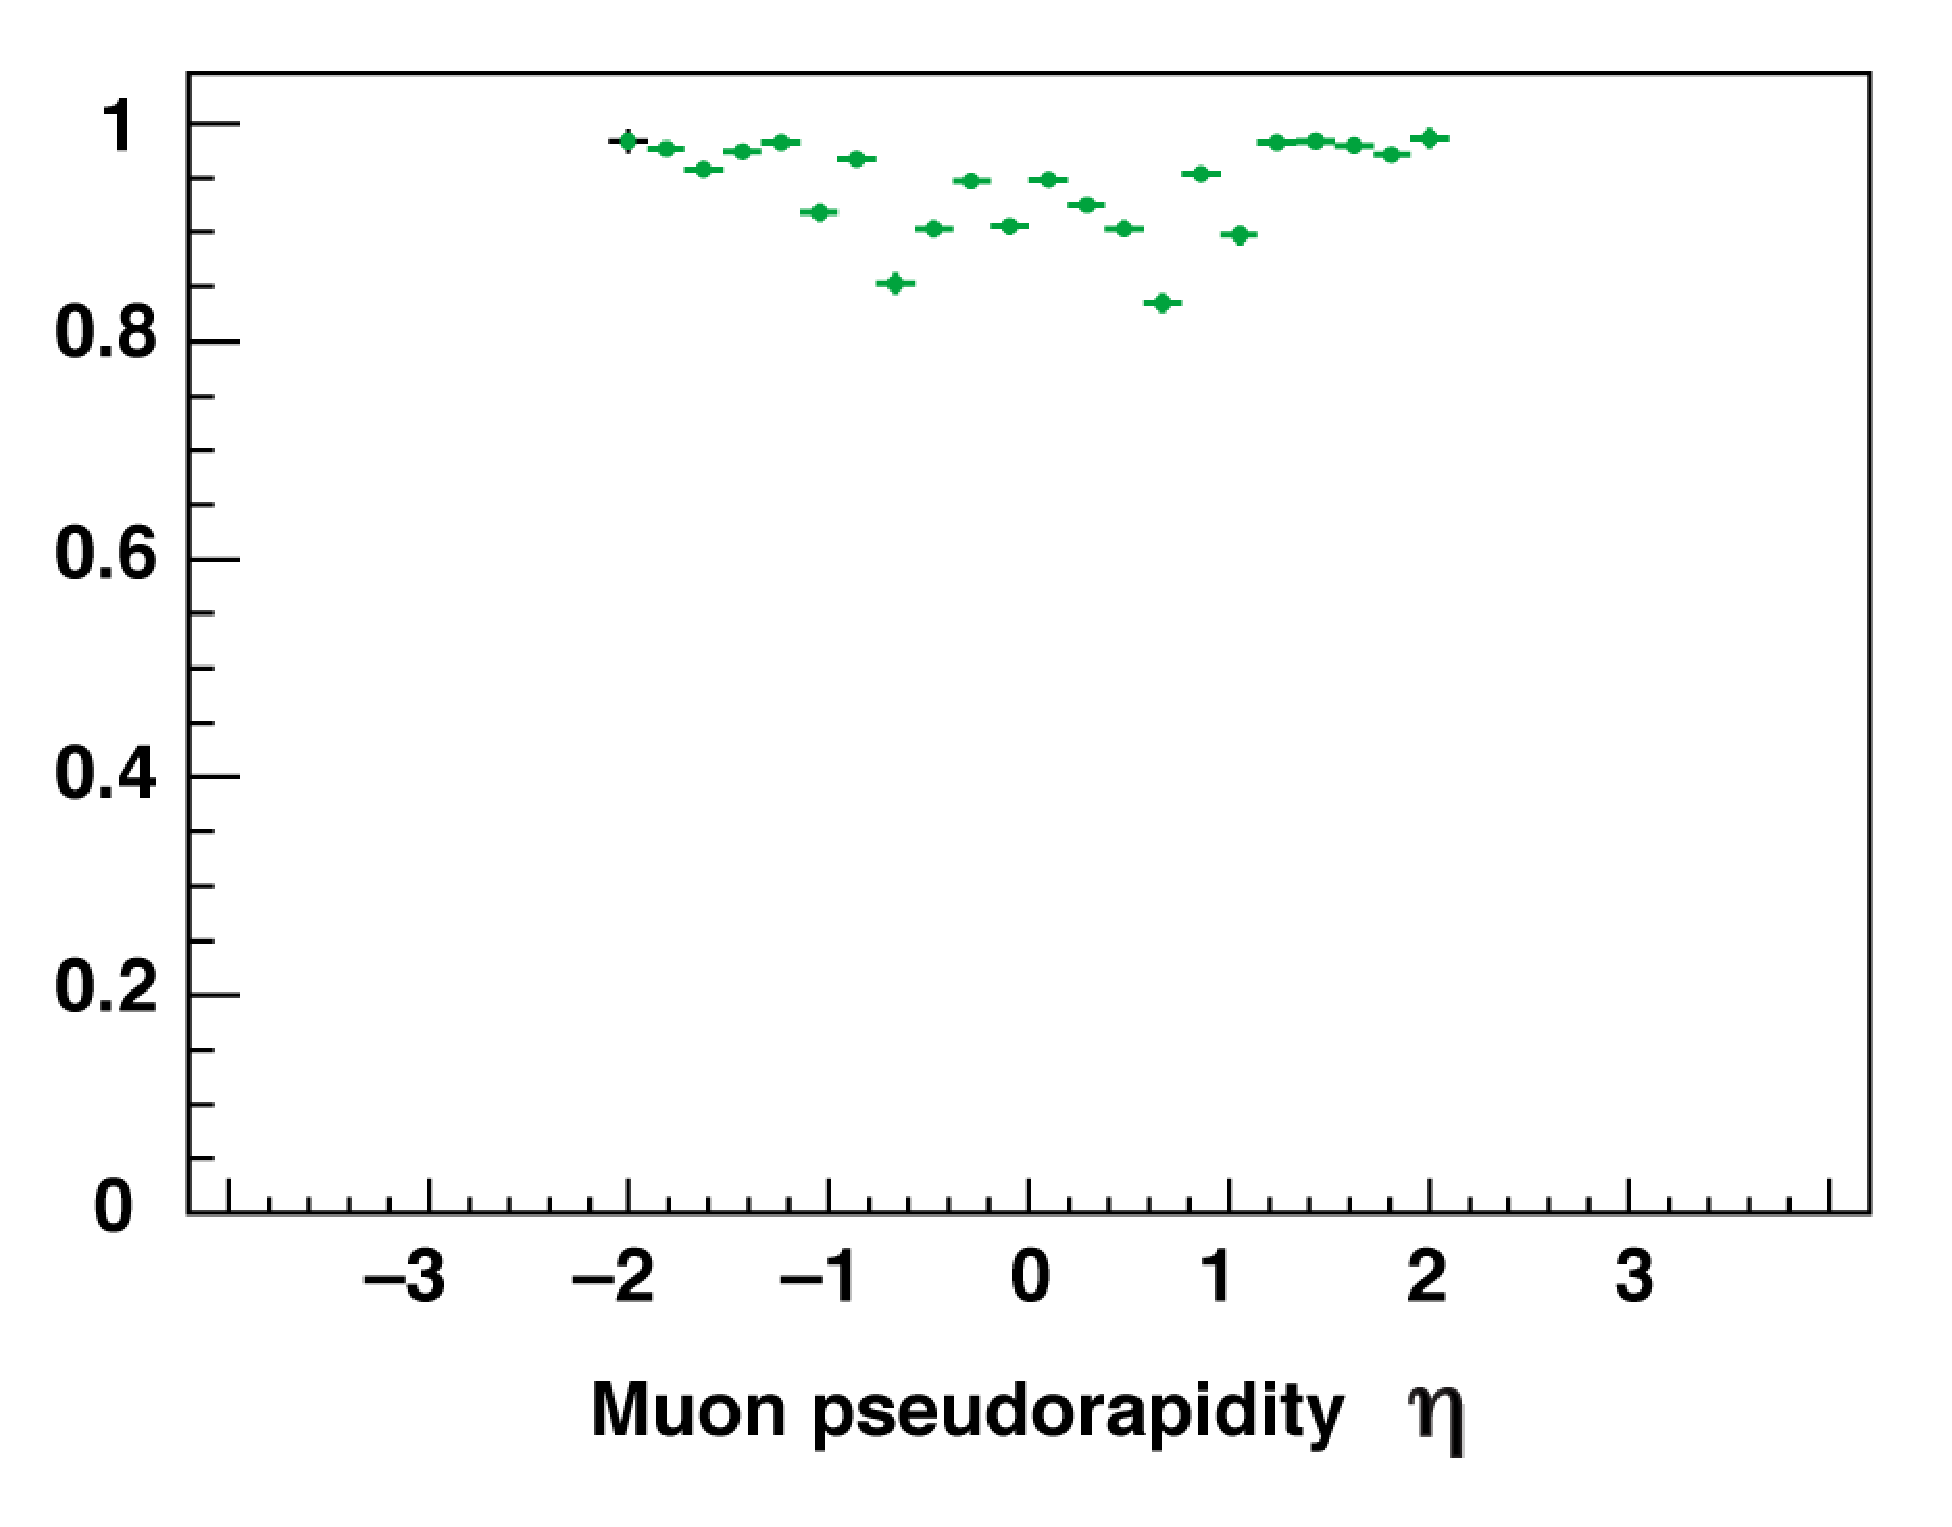
\includegraphics[width=0.35\textwidth]
{figures/muon_turn-on_curve_eta.eps}
\end{center}
\vspace{-0.1in}
\begin{minipage}{5.5in}
\caption[triggerturnons]{An example electron turn-on curve measured
as a function of the electron $p_T$ from trigger list v14 (left) and
an example muon turn-on curve measured as a function of {\deta} for
trigger lists v13--v15 (right). The muon curve is for Level 1 trigger
term mu1ptxatlx. The points are trigger efficiencies derived from data
in that bin (with uncertainty bars). The line is the corresponding fit
(for illustration purpose).}
\label{trigger-turnons}
\end{minipage}
\end{figure}

This analysis uses the ``caf\_trigger"~\cite{caf_trigger} package to
apply these turn-on curves to MC events. The caf\_trigger program
reads in turn-on curves for the number of physics objects (electrons,
muons, jets) in each event and the trigger list versions with the
associated integrated luminosities. It then uses ``processors'' to
perform combinatorics calculations and it then calculates the trigger
firing probabilities. Finally, it outputs a histogram of event
weights. The average efficiencies of $e$+jets and $\mu$+jets triggers
for signal events that pass selection are listed in
Tables~\ref{eltrigger-efficiencies} and
\ref{mutrigger-efficiencies}. These numbers are given for illustrative
purposes and are not used in the analysis.

\begin{table}[!h!tbp]
\begin{center}
\begin{minipage}{2.8in}
\begin{ruledtabular}
\begin{tabular}{c||cc} 
\multicolumn{3}{c}{\hspace{0.1in}\underline{Average Trigger Efficiencies}}\\
\multicolumn{3}{c}{\hspace{0.1in}\underline{in the Electron Channel}}\\
~~~ Trigger Version ~~~& $tb{\rar}e$+jets & $tqb{\rar}e$+jets \\
\hline
 v8.0 -- v9.0   &  92\%  &  92\%  \\            
 v9.0 -- v10.0  &  91\%  &  91\%  \\            
v10.0 -- v11.0  &  91\%  &  91\%  \\            
v11.0 -- v12.0  &  91\%  &  91\%  \\            
v12.0 -- v13.0  &  86\%  &  85\%  \\ 
v13.0 -- v13.3  &  87\%  &  86\%  \\            
v13.3 -- v14.0  &  86\%  &  85\%  \\         
v14.0 -- v15.0  &  88\%  &  87\%  \\
\hline		                
Overall average &  87\%  &  86\%
\end{tabular}
\end{ruledtabular}
\vspace{-0.1in}
\caption[eltriggerefficiencies]{Average electron-channel trigger
efficiencies for the single top events after selection.}
\label{eltrigger-efficiencies}
\end{minipage}
\end{center}
\end{table}


\begin{table}[!h!tbp]
\begin{center}
\begin{minipage}{2.8in}
\begin{ruledtabular}
\begin{tabular}{c||cc} 
\multicolumn{3}{c}{\hspace{0.1in}\underline{Average Trigger Efficiencies}}\\
\multicolumn{3}{c}{\hspace{0.1in}\underline{in the Muon Channel}}\\
~~~ Trigger Version ~~~& $tb{\rar}\mu$+jets & $tqb{\rar}\mu$+jets \\
\hline
 v8.0 -- v9.0   &  96\%  &  94\%  \\            
 v9.0 -- v10.0  &  93\%  &  90\%  \\            
v10.0 -- v11.0  &  91\%  &  88\%  \\            
v11.0 -- v12.0  &  92\%  &  88\%  \\            
v12.0 -- v13.0  &  91\%  &  88\%  \\ 
v13.0 -- v13.2  &  91\%  &  87\%  \\            
v13.2 -- v13.3  &  91\%  &  87\%  \\         
v13.3 -- v14.0  &  86\%  &  81\%  \\ 
v14.0 -- v14.2  &  92\%  &  89\%  \\   
v14.2 -- v14.3  &  92\%  &  89\%  \\
v14.3 -- v15.0  &  80\%  &  72\%  \\
\hline		                
Overall average &  87\%  &  82\%
\end{tabular}
\end{ruledtabular}
\vspace{-0.1in}
\caption[mutriggerefficiencies]{Average muon-channel trigger
efficiencies for the single top events after selection.}
\label{mutrigger-efficiencies}
\end{minipage}
\end{center}
\end{table}

\vspace{2in}